\documentclass[UTF8,a4paper,11pt]{ctexart}

\usepackage{geometry}
\usepackage{booktabs}
\usepackage{longtable}
\usepackage{array}
\usepackage{xcolor}
\usepackage{hyperref}
\usepackage{tabularx}
\usepackage{graphicx}
\usepackage{fvextra}
\usepackage{ragged2e}

\geometry{left=24mm,right=24mm,top=24mm,bottom=26mm}
\graphicspath{{assets/}{docs/reports/assets/}}
\hypersetup{
  colorlinks=true,
  linkcolor=blue!55!black,
  urlcolor=blue!55!black,
  citecolor=blue!55!black
}
\setlength{\parindent}{2em}
\setlength{\parskip}{0.42em}
\renewcommand{\arraystretch}{1.18}
\sloppy

\newcommand{\code}[1]{\texttt{\detokenize{#1}}}
\DefineVerbatimEnvironment{promptblock}{Verbatim}{fontsize=\scriptsize,breaklines=true,breakanywhere=true,frame=single,framesep=2mm}

\title{\bfseries OpenCollab SWE-bench G1.1 评测层重构报告}
\author{Codex}
\date{2026 年 7 月 8 日}

\begin{document}
\pagestyle{plain}
\maketitle

\begin{abstract}
这次工作做的是一件很具体的事：把 OpenCollab 里已经有价值的 SWE-bench 代码留住，把后来越写越乱的评测尝试隔开，然后重新做出一套能跑、能停、能看结果的 G1.1 评测层。G1.1 是版本号重置后的名字，它继承 V1 的 Validation Council 结构，并把编码尝试上限从两轮改为三轮。开发从 \code{cab511f} 起步，先用 \code{54a6c35} 保存可用基础，再补上状态判定、候选身份配对、有限损失恢复、只读状态观察、单命令 Pro-Lite runner、远端运行隔离、角色边界、工具空转控制、official eval 分类和短报告生成。此前用 G1.1 前身 V1 在 SWE-batch-pro-lite 第 26 到 35 题做过验证：10 道题全部生成 patch，10 道题都发起 official eval。其中 9 道题拿到有效语义结果，3 道题 resolved，6 道题 unresolved；第 32 题的 patch 已生成并进入评测，但 Redis 连接失败，按技术评测失败处理，需要在 Redis 正常后重评。
\end{abstract}

\section{重构起点}

重构先从找一个干净节点开始。\code{cab511f} 比较合适：它已经包含正式仓库 main 的合并结果，也保留了早期 SWE committee 和评测资料；它还没有卷入后面那些反复试 harness、反复卡住、反复宣称完成的复杂状态。基于这个节点创建 \code{54a6c35 建立评测重构前的可用基础}，把文档、会议资料、适配器和可复用测试先保存下来，然后在这块基础上开发 G1.1。

当时另一个线程正在评测单 Agent 25 题，所以重构写入放在独立 worktree 和独立分支上。这样正在跑的评测继续跑，G1.1 这边也有一条干净历史可以追。后面主工作区已经切回这条完成后的历史，当前 \code{main} 指向包含 G1.1 重构成果的工作区。

\section{开发目标}

G1.1 要解决的问题很朴素：给一组题号，脚本自己选题、生成 patch、识别非空 patch、触发 official eval、写报告，并且把“环境坏了”和“模型没解出来”分开。它继续搭在 OpenCollab 现有底层 harness 和高层 harness 上，沿用已有 workflow、远端 Docker 环境和 per-instance official eval 能力。

恢复能力也改成更现实的做法。G1.1 在生成阶段周期性保存 worktree diff，默认 300 秒一次；进程异常结束时，可以从最近保存的 patch 或显式失败状态继续处理。这里保护的是最终可评测 patch 和状态记录，没有把完整模型会话恢复当成前提。

\section{术语约定}

报告里把用户关心的自动评测小工具称为评测层。评测层处理题号切片、G1.1 runner、run directory、prediction 与 metric 配对、official eval、复评、状态读取和最终报告。它读取已经生成的 patch，也把评测结果写回机器可读 JSON、Markdown 和 PDF。

原有 harness 按层次分成底层 harness 和高层 harness。底层 harness 是单 Agent 能跑起来所需的基础能力，包括 provider 调用、会话运行、工具调用、文件读写、测试执行、超时处理、检查点和远端环境交互。高层 harness 是多 Agent 工作流，包括角色拆分、上下文拼接、并行角色、结构化输出校验、失败反馈和最终判定。

方向词也放在这里说清。下行表示任务、prompt、约束、工具权限、超时和预算从评测层或高层 harness 传给更低层；上行表示状态、证据、patch、日志、report 和 verdict 从底层 harness 或 agent 返回给更高层。后面定位 bug 时，会按评测层、底层 harness、高层 harness 归类，再说明问题发生在上行状态回传还是下行任务约束。

\section{G1.1 评测层架构详解}

G1.1 评测层外侧仍然有数据切片、runner、每题独立 run directory、official eval 与状态报告层。它们负责选题、启动、保存 patch、触发 official eval 和汇总状态。下面这张图只画高层 harness 里的 Validation Council，也就是 generation 阶段真正决定一个 patch 如何被分析、编写、验证和打回的 agent 结构。

\begin{figure}[htbp]
  \centering
  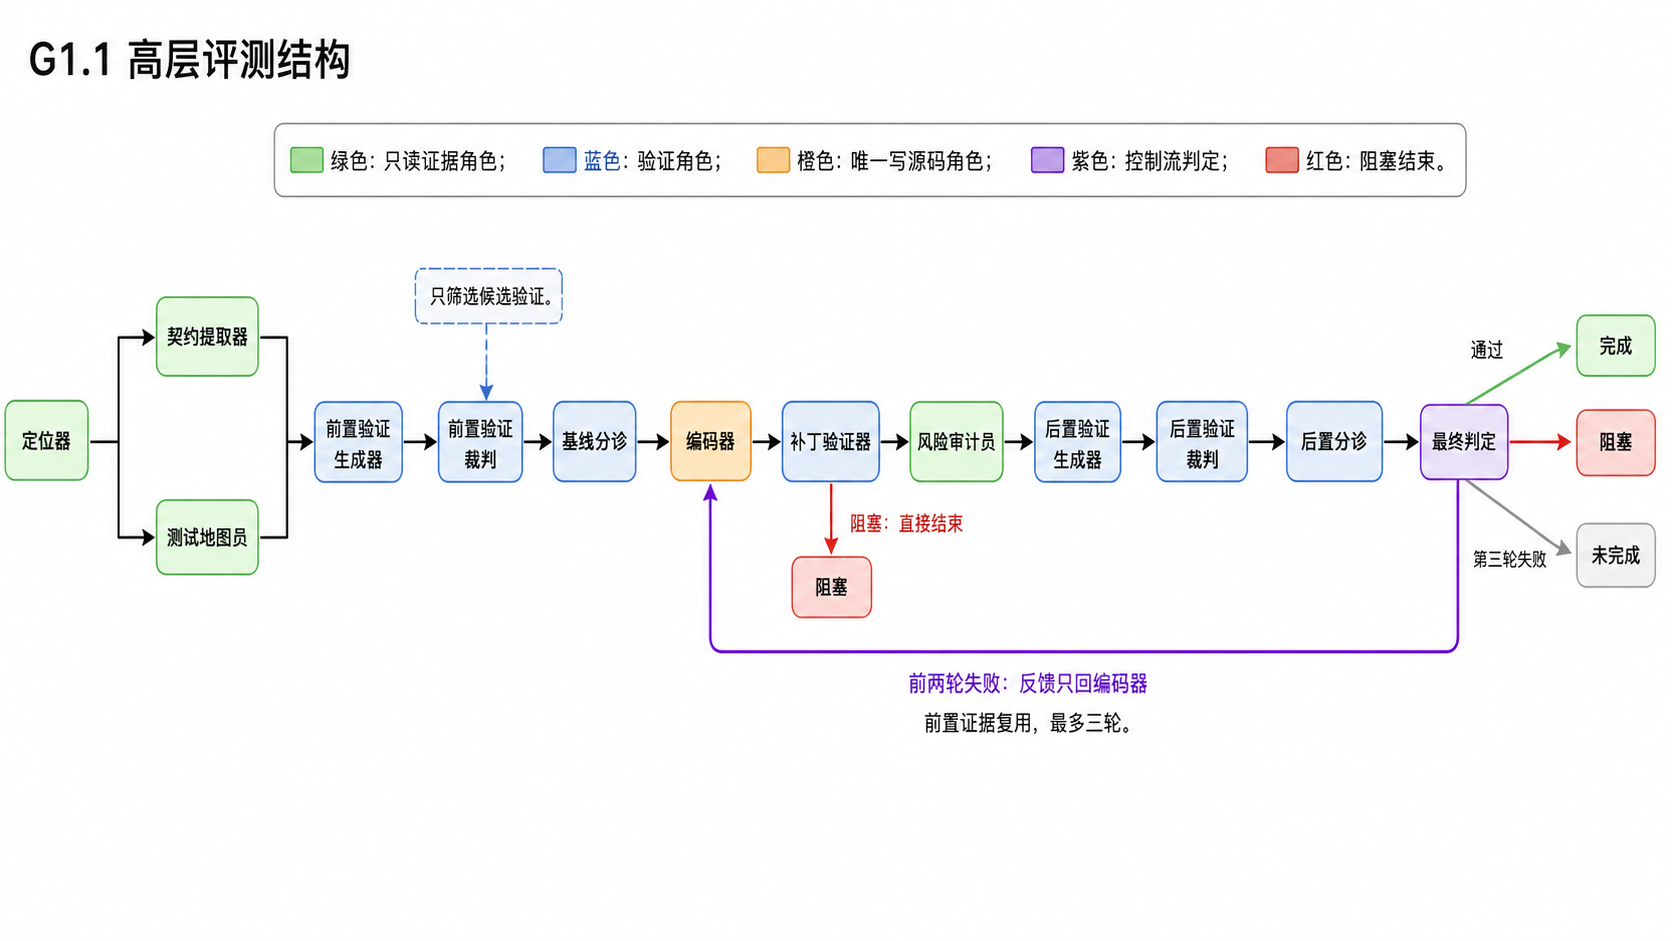
\includegraphics[width=\linewidth]{v1_harness_architecture.png}
  \caption{G1.1 高层 harness 的 agent 结构图。图中左侧是每题一次的证据准备，右侧是最多三轮的编码尝试；绿色角色做只读证据抽取，蓝色角色做验证，橙色编码器是唯一写入源码的角色，紫色表示控制流判定，红色表示阻塞结束。}
\end{figure}

图里的 agent flow 对应 \code{workflows/validation_council_solve.py}。每次 generation 开始时，workflow 从题目的 \code{goal} 或 \code{description} 取出问题描述。定位器先定位问题；契约提取器和测试地图员在 \code{ctx.parallel} 中并行运行；前置验证生成器生成候选验证；前置验证裁判过滤候选；基线分诊在改代码前运行廉价验证。这里得到的定位、契约、测试地图、候选验证和基线分类会作为后续尝试的共享证据，第一轮失败后不会重新跑这一段。

编码尝试区最多运行三轮。每一轮从编码器写 patch 开始，再经过补丁验证器、风险审计员、后置验证生成器、后置验证裁判、后置分诊和最终验证器。补丁验证器如果给出 \code{BLOCKED}，该轮会跳过后面的风险审查和后置验证，workflow 直接返回 \code{blocked}。最终验证器给 \code{PASS} 时返回 \code{done}；给 \code{BLOCKED} 时返回 \code{blocked}；第一轮或第二轮给 \code{FAIL} 时，workflow 会把最终验证器、补丁验证器、后置分诊和风险审计员的反馈拼成下一轮编码器的上下文。第三轮仍然 \code{FAIL} 时，workflow 返回 \code{incomplete}。这里确实有打回，但打回点只回到编码器，前置证据继续复用。

\subsection{通信协议与控制权}

G1.1 agent 之间没有点对点聊天。通信方式是中心调度：workflow 把上游结果整理进下游 prompt，带 schema 的角色再通过 \code{structured_output} 返回 JSON。每个角色都由 \code{ctx.agent(prompt, schema=..., label=..., tools=..., budget=..., timeout=...)} 启动。runtime 校验 JSON Schema；如果校验失败，或者某个 agent 死亡，workflow 会把结果视为 \code{None}，随后用 fallback 字典继续跑。这样单个角色出问题时，损失的是这一步证据质量，整个 workflow 仍然能给出 done、blocked 或 incomplete 状态。

从“谁把消息给谁”看，定位器的输出只回到 workflow；workflow 再把它发给契约提取器和测试地图员。契约提取器和测试地图员互相不通信，它们的结果在 workflow 里合并后发给前置验证生成器。前置验证生成器把候选验证交回 workflow，workflow 发给前置验证裁判；前置验证裁判的 accepted 列表会进入基线分诊、编码器、补丁验证器和最终验证器。编码器的源码改动留在工作树里，文字报告回到 workflow 后发给补丁验证器和最终验证器。补丁验证器的 verdict 发给风险审计员和最终验证器；风险审计员的 risks 发给后置验证生成器和最终验证器；后置验证裁判的结果发给后置分诊；后置分诊的结果发给最终验证器。

从“谁能决定走向”看，前置验证裁判和后置验证裁判只负责筛选验证候选，不结束 workflow，也不触发回退。编码器能改源码，但不能决定是否进入下一轮。补丁验证器只有在给出 \code{BLOCKED} 时改变控制流：workflow 会立即返回 \code{blocked}。补丁验证器给 \code{PASS} 或 \code{FAIL} 时，它的结论只作为后续角色的证据。真正决定 done、blocked、重试和 incomplete 的角色是最终验证器；workflow 再结合 \code{MAX_CODER_ROUNDS = 3} 决定第一轮或第二轮失败后打回编码器，或第三轮失败后返回 \code{incomplete}。

上下文传递尽量短。定位器只吃原始 \code{goal}；契约提取器和测试地图员吃 \code{goal + localization}；前置验证生成器吃 \code{goal + localization + contracts + cartography}；裁判吃 \code{goal + contracts + candidates}；基线分诊吃 \code{goal + accepted validation}；编码器吃所有前置证据和上一轮反馈；补丁验证器吃编码器报告、pre-judge 和 baseline triage；风险审计员只吃 contracts 和 patch verdict；后置验证生成器吃 contracts 和 diff risks；后置分诊吃 post judge；最终验证器吃本轮全部结构化证据。

工具权限和通信协议绑在一起。只读角色使用 \code{FileReadTool} 和 \code{GrepTool}；Coder 使用 \code{BashTool}、\code{FileReadTool}、\code{FileWriteTool}、\code{ApplyPatchTool}、\code{RunTestsTool} 和 \code{GrepTool}；验证角色使用 \code{FileReadTool}、受限 \code{RunTestsTool}、\code{GrepTool} 和 \code{GitDiffTool}；Risk Auditor 没有工具。共享规则要求所有角色只看 issue、仓库代码、公开测试和公开文档；临时验证只能放在 \code{/tmp/opencollab-validation-*}；最终 diff 不能包含临时文件、测试污染、日志、缓存或笔记。

Schema 的边界也写死在代码里。Localizer 输出问题摘要、根因假设、相关文件、公开 API、未知项和完成条件；Contract Miner 输出带证据的行为契约；Candidate schema 输出候选验证、契约 id、oracle、setup、断言、base/patch 期望和误报风险；Judge schema 输出 accepted、rejected、diagnostic 和 validation brief；Triage schema 输出每个验证的分类与证据；Risk schema 输出最多三个风险；Verdict schema 输出 \code{PASS}、\code{FAIL} 或 \code{BLOCKED}，再附 allowed 与 disallowed patch paths。

\subsection{Agent 参数、通信和完整 Prompt}

运行时 prompt 来自代码里的模板，执行 \code{format(...)} 后才变成真正发给模型的文本。下面保留模板中的动态占位符，例如 \code{{goal}}、\code{{contracts}} 和 \code{{patch_verdict}}；运行时会用题目描述或上游 agent 的 JSON 结果替换它们。Agent 之间没有直接寻址发送接口；每个 agent 的输出先回到 workflow，再由 workflow 放进后续 prompt 或写入 attempt 结果。带 \code{schema=} 的 agent 必须调用 \code{structured_output}，runtime 校验 JSON Schema 后返回 dict；Coder 没有 \code{schema=}，返回普通 final text，死亡或无返回时由 workflow 当作空字符串处理。

\begingroup
\RaggedRight

\paragraph{Analyst / Localizer.}
这个角色的 label 是 \code{analyst-localizer}，prompt 是 \code{LOCALIZER_PROMPT}，schema 是 \code{LOCALIZATION_SCHEMA}。它只能使用 \code{FileReadTool} 和 \code{GrepTool}，budget 为 \code{220000}，timeout 为 \code{300} 秒。输入只有 \code{goal} 和 \code{SHARED_RULES}；输出会作为 \code{localization} 传给 Contract Miner、Test Cartographer、Pre-Validation Factory、Coder 和 Final Verifier。返回对象必须包含 \code{summary}、\code{root_cause_hypothesis}、\code{files}、\code{public_api}、\code{uncertainties} 和 \code{definition_of_done}。

\paragraph{Contract Miner.}
这个角色的 label 是 \code{contract-miner}，prompt 是 \code{CONTRACT_MINER_PROMPT}，schema 是 \code{CONTRACT_SCHEMA}。它用 \code{FileReadTool} 和 \code{GrepTool} 读证据，budget 为 \code{180000}，timeout 为 \code{300} 秒。输入是 \code{goal}、\code{localization} 和 \code{SHARED_RULES}；它会和 Test Cartographer 在 \code{ctx.parallel} 中并行。输出作为 \code{contracts} 传给 Pre-Validation Factory、Judge、Coder、Risk Auditor、Post-Validation Factory 和 Final Verifier。返回值必须包含 \code{contracts} 数组；每条契约包含 \code{id}、\code{statement}、\code{scope}、\code{behavior_kind}、\code{evidence}、\code{confidence} 和 \code{testability}。

\paragraph{Test Cartographer.}
这个角色的 label 是 \code{test-cartographer}，prompt 是 \code{TEST_CARTOGRAPHER_PROMPT}，schema 是 \code{TEST_CARTOGRAPHY_SCHEMA}。它使用 \code{FileReadTool} 和 \code{GrepTool}，budget 为 \code{180000}，timeout 为 \code{300} 秒。输入是 \code{goal}、\code{localization} 和 \code{SHARED_RULES}；它与 Contract Miner 并行。输出作为 \code{cartography} 传给 Pre-Validation Factory 和 Coder。返回值必须包含 \code{framework}、\code{runner_commands}、\code{test_files}、\code{fixtures}、\code{assertion_style} 和 \code{temporary_test_guidance}。

\paragraph{Pre-Patch Validation Factory.}
这个角色的 label 是 \code{pre-validation-factory}，prompt 是 \code{PRE_VALIDATION_FACTORY_PROMPT}，schema 是 \code{CANDIDATE_TESTS_SCHEMA}。它使用 \code{FileReadTool} 和 \code{GrepTool}，budget 为 \code{160000}，timeout 为 \code{300} 秒。输入包括 \code{goal}、\code{localization}、\code{contracts}、\code{cartography} 和 \code{SHARED_RULES}；输出作为 \code{candidates} 交给 pre-stage Validation Judge。返回值必须包含 \code{tests}、\code{abstained} 和 \code{rationale}；每个候选测试必须带 contract id、oracle、setup、assertion、base/patch 期望和误报风险。

\paragraph{Validation Judge / Prioritizer.}
\code{_judge_candidates} 统一创建这个角色。pre 阶段 label 是 \code{pre-validation-judge}，post 阶段 label 是 \code{post-rN-validation-judge}；prompt 是 \code{JUDGE_PROMPT}；schema 是 \code{JUDGE_SCHEMA}；工具是 \code{FileReadTool} 与 \code{GrepTool}；budget 为 \code{100000}；timeout 为 \code{300} 秒。它接收 \code{goal}、\code{contracts}、\code{candidates}、\code{stage}、\code{cap} 和 \code{SHARED_RULES}。pre 阶段输出 \code{pre_judge}，后续给 Baseline Triage、Coder、Patch Validator 和 Final Verifier；post 阶段输出 \code{post_judge}，后续给 Post Triage 和 Final Verifier。返回值必须包含 \code{accepted}、\code{rejected}、\code{diagnostic} 和 \code{validation_brief}；pre 阶段 cap 是 \code{5}，post 阶段 cap 是 \code{4}，workflow 还会用 \code{_trim_judge} 再截断。

\paragraph{Baseline Executor and Triage.}
这个角色的 label 是 \code{baseline-triage}，prompt 是 \code{BASELINE_TRIAGE_PROMPT}，schema 是 \code{TRIAGE_SCHEMA}。它使用 \code{FileReadTool}、\code{RunTestsTool}、\code{GrepTool} 与 \code{GitDiffTool}；其中 \code{RunTestsTool} 的参数是 \code{allow_runner_override=False} 和 \code{allow_extra_args=False}。budget 为 \code{180000}，timeout 为 \code{300} 秒。它接收 \code{goal}、\code{pre_judge} 和 \code{SHARED_RULES}；输出作为 \code{baseline_triage} 传给 Coder、Patch Validator 和 Final Verifier。返回值必须包含 \code{classifications}、\code{approved_brief} 和 \code{abstained}；分类状态来自 \code{base_fail_repro}、\code{base_pass_regression}、\code{patch_pass}、\code{patch_fail}、\code{invalid}、\code{weak} 和 \code{not_run}。

\paragraph{Coder.}
Coder 是唯一能写源码的角色。它的 label 是 \code{coder:rN}，prompt 是 \code{CODER_PROMPT}；如果有上一轮反馈，workflow 会追加 \code{FEEDBACK_BLOCK}。它没有 schema，工具是 \code{BashTool}、\code{FileReadTool}、\code{FileWriteTool}、\code{ApplyPatchTool}、\code{RunTestsTool} 和 \code{GrepTool}；budget 未传入，timeout 为 \code{1800} 秒。它接收 \code{goal}、\code{localization}、\code{contracts}、\code{cartography}、\code{pre_judge}、\code{baseline_triage}、\code{feedback_block} 和 \code{SHARED_RULES}。输出作为 \code{coder_report} 传给 Patch Validator 和 Final Verifier。由于它返回普通文本，workflow 会用 \code{coder_report or "(coder returned no report)"} 处理空返回。

\paragraph{Patch Validator.}
这个角色的 label 是 \code{patch-validator:rN}，prompt 是 \code{PATCH_VALIDATOR_PROMPT}，schema 是 \code{VERDICT_SCHEMA}。它使用 \code{FileReadTool}、\code{RunTestsTool}、\code{GrepTool} 与 \code{GitDiffTool}；其中 \code{RunTestsTool} 的参数是 \code{allow_runner_override=False} 和 \code{allow_extra_args=False}。budget 为 \code{220000}，timeout 为 \code{300} 秒。它接收 \code{goal}、\code{coder_report}、\code{pre_judge}、\code{baseline_triage} 和 \code{SHARED_RULES}。输出 \code{patch_verdict} 会传给 Diff Risk Auditor、Final Verifier 和失败反馈；若 verdict 是 \code{BLOCKED}，该 attempt 直接用这个 verdict 返回。返回值必须包含 \code{verdict}、\code{findings}、\code{allowed_patch_paths} 和 \code{disallowed_patch_paths}；verdict 枚举为 \code{PASS}、\code{FAIL} 和 \code{BLOCKED}。

\paragraph{Diff Risk Auditor.}
这个角色的 label 是 \code{diff-risk-auditor:rN}，prompt 是 \code{DIFF_RISK_PROMPT}，schema 是 \code{DIFF_RISK_SCHEMA}。它没有工具，budget 为 \code{60000}，timeout 为 \code{300} 秒。它接收 \code{goal}、\code{contracts}、\code{patch_verdict} 和 \code{SHARED_RULES}。输出 \code{risks} 传给 Post-Patch Validation Factory、Final Verifier 和失败反馈。返回值必须包含 \code{risks} 和 \code{summary}；每个 risk 包含 \code{id}、\code{changed_area}、\code{risk}、\code{contract_ids}、\code{suggested_probe} 和 \code{priority}。

\paragraph{Post-Patch Validation Factory.}
这个角色的 label 是 \code{post-validation-factory:rN}，prompt 是 \code{POST_VALIDATION_FACTORY_PROMPT}，schema 是 \code{CANDIDATE_TESTS_SCHEMA}。它使用 \code{FileReadTool} 与 \code{GrepTool}，budget 为 \code{160000}，timeout 为 \code{300} 秒。它接收 \code{goal}、\code{contracts}、\code{risks} 和 \code{SHARED_RULES}。输出作为 \code{post_candidates} 传给 post-stage Validation Judge。输出结构与 pre validation factory 相同，必须返回 \code{tests}、\code{abstained} 和 \code{rationale}。

\paragraph{Post-Patch Validation Triage.}
这个角色的 label 是 \code{post-validation-triage:rN}，prompt 是 \code{POST_TRIAGE_PROMPT}，schema 是 \code{TRIAGE_SCHEMA}。它使用 \code{FileReadTool}、\code{RunTestsTool}、\code{GrepTool} 与 \code{GitDiffTool}；其中 \code{RunTestsTool} 的参数是 \code{allow_runner_override=False} 和 \code{allow_extra_args=False}。budget 为 \code{180000}，timeout 为 \code{300} 秒。它接收 \code{goal}、\code{post_judge} 和 \code{SHARED_RULES}。输出 \code{post_triage} 传给 Final Verifier 和失败反馈。返回值必须包含 \code{classifications}、\code{approved_brief} 和 \code{abstained}；post 场景常用状态是 \code{patch_pass}、\code{patch_fail}、\code{invalid}、\code{weak} 和 \code{not_run}。

\paragraph{Final Verifier.}
这个角色的 label 是 \code{final-verifier:rN}，prompt 是 \code{FINAL_VERIFIER_PROMPT}，schema 是 \code{VERDICT_SCHEMA}。它使用 \code{FileReadTool}、\code{RunTestsTool}、\code{GrepTool} 与 \code{GitDiffTool}；其中 \code{RunTestsTool} 的参数是 \code{allow_runner_override=False} 和 \code{allow_extra_args=False}。budget 为 \code{220000}，timeout 为 \code{300} 秒。它接收 \code{goal}、\code{localization}、\code{contracts}、\code{pre_judge}、\code{baseline_triage}、\code{coder_report}、\code{patch_verdict}、\code{risks}、\code{post_judge}、\code{post_triage} 和 \code{SHARED_RULES}。输出 \code{final_verdict} 决定 workflow 返回 \code{done}、\code{blocked} 或 \code{incomplete}，失败时也会进入下一轮 Coder 的 feedback。返回值必须包含 \code{verdict}、\code{findings}、\code{allowed_patch_paths} 和 \code{disallowed_patch_paths}；只有 \code{PASS} 会让 workflow 返回 \code{status=done}。

\subsubsection*{结构化输出 Schema 约束}

所有带 \code{schema=} 的角色都通过 \code{structured_output} 返回 JSON。schema 校验失败时，runtime 会在同一 session 做一次纠正重试；仍失败时返回 \code{None}，workflow 随后使用代码里定义的 fallback dict 继续执行。这个部分偏参考手册，放在这里是为了让后续修改 prompt 或 schema 时有一份能直接对照的说明。

\paragraph{LOCALIZATION\_SCHEMA.}
顶层必填 \code{summary}、\code{root_cause_hypothesis}、\code{files}、\code{public_api}、\code{uncertainties} 和 \code{definition_of_done}；其中 \code{files}、\code{public_api} 与 \code{uncertainties} 是字符串数组。

\paragraph{CONTRACT\_SCHEMA.}
顶层必填 \code{contracts}；每条契约必填 \code{id}、\code{statement}、\code{scope}、\code{behavior_kind}、\code{evidence}、\code{confidence} 和 \code{testability}。\code{behavior_kind} 枚举为 \code{desired}、\code{current_buggy} 和 \code{existing_unaffected}。\code{evidence} 中每项必填 \code{source_type}、\code{file_or_section} 和 \code{summary}。

\paragraph{TEST\_CARTOGRAPHY\_SCHEMA.}
顶层必填 \code{framework}、\code{runner_commands}、\code{test_files}、\code{fixtures}、\code{assertion_style} 和 \code{temporary_test_guidance}；其中 \code{runner_commands}、\code{test_files} 与 \code{fixtures} 是字符串数组。

\paragraph{CANDIDATE\_TESTS\_SCHEMA.}
顶层必填 \code{tests}、\code{abstained} 和 \code{rationale}。每个测试必填 \code{id}、\code{contract_ids}、\code{type}、\code{oracle_type}、\code{setup}、\code{assertion}、\code{expected_on_base}、\code{expected_on_patch}、\code{why_distinguishes_wrong_patch}、\code{evidence_refs}、\code{runner_command} 和 \code{risk_of_false_positive}。\code{type} 枚举为 \code{repro}、\code{edge}、\code{regression}、\code{metamorphic} 和 \code{diagnostic}；\code{expected_on_base} 枚举为 \code{fail}、\code{pass} 和 \code{unknown}；\code{expected_on_patch} 枚举为 \code{pass} 和 \code{unknown}。

\paragraph{JUDGE\_SCHEMA.}
顶层必填 \code{accepted}、\code{rejected}、\code{diagnostic} 和 \code{validation_brief}。\code{accepted} 每项必填 \code{id}、\code{priority}、\code{classification} 和 \code{reason}；\code{rejected} 每项必填 \code{id} 和 \code{reason}。

\paragraph{TRIAGE\_SCHEMA.}
顶层必填 \code{classifications}、\code{approved_brief} 和 \code{abstained}。\code{classifications} 每项必填 \code{test_id}、\code{status} 和 \code{evidence}；\code{status} 枚举为 \code{base_fail_repro}、\code{base_pass_regression}、\code{patch_pass}、\code{patch_fail}、\code{invalid}、\code{weak} 和 \code{not_run}。

\paragraph{DIFF\_RISK\_SCHEMA.}
顶层必填 \code{risks} 和 \code{summary}。\code{risks} 每项必填 \code{id}、\code{changed_area}、\code{risk}、\code{contract_ids}、\code{suggested_probe} 和 \code{priority}。

\paragraph{VERDICT\_SCHEMA.}
顶层必填 \code{verdict}、\code{findings}、\code{allowed_patch_paths} 和 \code{disallowed_patch_paths}。\code{verdict} 枚举为 \code{PASS}、\code{FAIL} 和 \code{BLOCKED}；两个 path 字段都是字符串数组。

\endgroup

\subsubsection*{共享规则完整文本}

\begin{promptblock}
Rules:
- Use only the issue text, repository code, public tests, and public docs.
- Do not use hidden grader tests, official test patches, injected FAIL_TO_PASS
  node ids, or any task extra that reveals the grading suite.
- Prefer dedicated tools: file_read/grep for inspection, run_tests for tests,
  file_write/apply_patch for edits. Use bash only when no dedicated tool fits.
- Keep temporary validation outside the final diff. Do not edit tests unless the
  task explicitly asks for a test-only change.
- Only roles with command or write tools may create temporary validation files.
  If your current tools cannot create or run a probe, report that limitation in
  structured_output instead of searching for unavailable tools.
- If a validation probe needs a temporary file and your role has a tool that can
  create it, write it only under /tmp/opencollab-validation-* and remove it
  after use.
- Fix the source root cause with the smallest correct change.
- Never run git commit; leave edits in the working tree.
\end{promptblock}

\subsubsection*{LOCALIZER\_PROMPT}

\begin{promptblock}
You are the Analyst / Localizer. Analyze only; do not edit files.
Identify the likely source area, public API, root-cause hypothesis, unknowns,
and definition of done. Read the repository and public tests for evidence.

{rules}

Goal:
{goal}
\end{promptblock}

\subsubsection*{CONTRACT\_MINER\_PROMPT}

\begin{promptblock}
You are the Contract Miner. Extract behavior contracts only. A contract must be
grounded in issue text, source behavior, public docs, or public tests. Do not
write tests and do not infer exact hidden assertions.

For each contract, record whether it describes desired behavior, currently
buggy behavior, or existing unaffected behavior. Cite concrete evidence.

{rules}

Goal:
{goal}

Localization:
{localization}
\end{promptblock}

\subsubsection*{TEST\_CARTOGRAPHER\_PROMPT}

\begin{promptblock}
You are the Test Cartographer. Map how this repository expresses tests: runner,
fixtures, assertion style, relevant public test files, and how temporary probes
can be run without entering the final diff. Do not solve the issue.

{rules}

Goal:
{goal}

Localization:
{localization}
\end{promptblock}

\subsubsection*{PRE\_VALIDATION\_FACTORY\_PROMPT}

\begin{promptblock}
You are the Pre-Patch Validation Factory. Propose candidate validation probes
before coding. Each candidate must link to behavior contract ids and evidence.
Prefer short repro, boundary, regression, or metamorphic probes. Mark weak or
diagnostic-only probes as such. Do not edit files, do not run probes, and do not
look for write tools. If evidence is insufficient, set abstained=true.

{rules}

Goal:
{goal}

Localization:
{localization}

Contracts:
{contracts}

Test cartography:
{cartography}
\end{promptblock}

\subsubsection*{JUDGE\_PROMPT}

\begin{promptblock}
You are the Validation Judge / Prioritizer for the {stage} stage. Apply hard
evidence gates. Accept at most {cap} candidates. Reject a candidate if it lacks
contract ids, lacks concrete evidence, asserts behavior only from a proposed
implementation, or depends on hidden grader knowledge. Diagnostics may be kept
separate, but they must not block final acceptance. Do not edit files, do not
create temporary probes, and do not look for write tools.

{rules}

Goal:
{goal}

Contracts:
{contracts}

Candidates:
{candidates}
\end{promptblock}

\subsubsection*{BASELINE\_TRIAGE\_PROMPT}

\begin{promptblock}
You are the Baseline Executor and Triage role. Run only accepted validation
probes that are cheap and safe, using temporary files or one-shot commands that
do not enter the final diff. If a file is needed, use /tmp/opencollab-validation-*
only when the provided tools can create it. If the provided tools cannot run a
probe exactly, classify it as not_run or weak instead of searching for missing
tools. Classify each accepted probe against the current base as base_fail_repro,
base_pass_regression, invalid, weak, or not_run. Record exact commands and
observations.

{rules}

Goal:
{goal}

Accepted validation:
{judge}
\end{promptblock}

\subsubsection*{CODER\_PROMPT}

\begin{promptblock}
You are the Coder. Implement a minimal source fix using the evidence package.
Do not edit tests unless the task explicitly requires test-only changes.
Run relevant public tests and accepted validation probes where practical.
Once you can name the concrete source change, stop reading and call file_write
or apply_patch in that turn. Do not announce an edit and then call file_read or
grep.
Your final message should name changed source files, explain the root cause,
and summarize verification.

{rules}

Goal:
{goal}

Localization:
{localization}

Contracts:
{contracts}

Test cartography:
{cartography}

Pre-patch validation judge:
{pre_judge}

Baseline triage:
{baseline_triage}
{feedback_block}
\end{promptblock}

\subsubsection*{FEEDBACK\_BLOCK}

\begin{promptblock}

Previous attempt feedback:
{feedback}
\end{promptblock}

\subsubsection*{PATCH\_VALIDATOR\_PROMPT}

\begin{promptblock}
You are the Patch Validator. Do not edit files. Verify the current working tree
against the goal, public tests, accepted pre-patch validation, and baseline
triage. Run existing tests when practical; do not create new probe files and do
not search for write tools. If a requested probe cannot be run with available
tools, say so in findings. Verdict PASS only when the source change is present,
minimal, and satisfies the approved validation. Run `git diff --name-only`; put
legitimate source paths in allowed_patch_paths and all tests, temporary probes,
caches, logs, notes, and generated artifacts in disallowed_patch_paths.

{rules}

Goal:
{goal}

Coder report:
{coder_report}

Accepted validation:
{pre_judge}

Baseline triage:
{baseline_triage}
\end{promptblock}

\subsubsection*{DIFF\_RISK\_PROMPT}

\begin{promptblock}
You are the Diff Risk Auditor. Do not edit files and do not run tools. Use only
the contracts and patch validator verdict already provided below. Identify at
most three semantic risks, missed contracts, neighboring behavior that may
regress, and focused probes that would catch those risks. If the verdict already
contains enough clean evidence, return an empty risks list with a concise
summary. Do not inspect more repository files. Your next action must be
structured_output.

{rules}

Goal:
{goal}

Contracts:
{contracts}

Patch validator verdict:
{patch_verdict}
\end{promptblock}

\subsubsection*{POST\_VALIDATION\_FACTORY\_PROMPT}

\begin{promptblock}
You are the Post-Patch Validation Factory. Use the accepted contracts, current
diff risks, and public repository behavior to propose additional post-patch
probes. Do not derive assertions only from the implementation. Do not edit
files, do not run probes, and do not look for write tools. If risks are empty or
evidence is insufficient, set abstained=true.

{rules}

Goal:
{goal}

Contracts:
{contracts}

Diff risks:
{risks}
\end{promptblock}

\subsubsection*{POST\_TRIAGE\_PROMPT}

\begin{promptblock}
You are the Post-Patch Validation Triage role. Run accepted post-patch probes
when cheap and safe. Keep temporary probes outside the final diff. Classify each
probe as patch_pass, patch_fail, invalid, weak, or not_run. If a file is needed,
use /tmp/opencollab-validation-* only when the provided tools can create it. If
the provided tools cannot run a probe exactly, classify it as not_run or weak
instead of searching for missing tools. Report exact commands and observations.

{rules}

Goal:
{goal}

Accepted post-patch validation:
{judge}
\end{promptblock}

\subsubsection*{FINAL\_VERIFIER\_PROMPT}

\begin{promptblock}
You are the Final Verifier. Do not edit files. Inspect git diff, run relevant
public tests and approved validation where practical, and check that temporary
validation files are absent from the final diff. Run existing tests when
practical; do not create new probe files and do not search for write tools. Run
`git diff --name-only` and place legitimate source changes in allowed_patch_paths.
Place all tests, temporary probes, caches, logs, notes, and generated artifacts
in disallowed_patch_paths, and fail if any disallowed path remains in the diff.
Verdict PASS only when the issue is fixed by source changes and the validation
evidence is clean.

{rules}

Goal:
{goal}

Localization:
{localization}

Contracts:
{contracts}

Pre-patch validation:
{pre_judge}

Baseline triage:
{baseline_triage}

Coder report:
{coder_report}

Patch validator verdict:
{patch_verdict}

Diff risks:
{risks}

Post-patch validation:
{post_judge}

Post-patch triage:
{post_triage}
\end{promptblock}

\subsection{Agent Prompt 中文版}

下面给出同一组 prompt 的中文译文，便于直接阅读。运行时模板仍以上面的英文原文展示，动态占位符如 \code{{goal}}、\code{{contracts}}、\code{{patch_verdict}} 保持原样。

\subsubsection*{共享规则中文版}

\begin{promptblock}
规则：
- 只使用 issue 文本、仓库代码、公开测试和公开文档。
- 不使用隐藏评分测试、官方测试 patch、注入的 FAIL_TO_PASS 节点 id，
  也不使用任何会透露评分套件的任务额外信息。
- 优先使用专用工具：file_read/grep 用于检查，run_tests 用于测试，
  file_write/apply_patch 用于编辑。只有在没有合适专用工具时才使用 bash。
- 临时验证必须留在最终 diff 之外。除非任务明确要求只改测试，
  否则不要编辑测试。
- 只有拥有命令工具或写入工具的角色可以创建临时验证文件。如果当前工具
  不能创建或运行 probe，就在 structured_output 中报告这个限制，
  不要搜索不存在的工具。
- 如果验证 probe 需要临时文件，并且当前角色有工具可以创建它，
  只能写到 /tmp/opencollab-validation-* 下面，用完后删除。
- 用最小且正确的改动修复源码根因。
- 永远不要运行 git commit；把编辑留在工作树里。
\end{promptblock}

\subsubsection*{LOCALIZER\_PROMPT 中文版}

\begin{promptblock}
你是 Analyst / Localizer。只做分析；不要编辑文件。
识别可能的源码区域、公开 API、根因假设、未知项和完成条件。
阅读仓库和公开测试来获得证据。

{rules}

目标：
{goal}
\end{promptblock}

\subsubsection*{CONTRACT\_MINER\_PROMPT 中文版}

\begin{promptblock}
你是 Contract Miner。只抽取行为契约。契约必须基于 issue 文本、
源码行为、公开文档或公开测试。不要写测试，也不要推断隐藏断言的精确内容。

对每条契约，记录它描述的是期望行为、当前有 bug 的行为，
还是已有且不受影响的行为。引用具体证据。

{rules}

目标：
{goal}

定位结果：
{localization}
\end{promptblock}

\subsubsection*{TEST\_CARTOGRAPHER\_PROMPT 中文版}

\begin{promptblock}
你是 Test Cartographer。梳理这个仓库如何表达测试：runner、
fixtures、断言风格、相关公开测试文件，以及如何运行临时 probe
并确保它们不进入最终 diff。不要解题。

{rules}

目标：
{goal}

定位结果：
{localization}
\end{promptblock}

\subsubsection*{PRE\_VALIDATION\_FACTORY\_PROMPT 中文版}

\begin{promptblock}
你是 Pre-Patch Validation Factory。在编码前提出候选验证 probe。
每个候选项必须链接到行为契约 id 和证据。优先选择短小的复现、
边界、回归或变形 probe。把弱 probe 或仅诊断用 probe 标出来。
不要编辑文件，不要运行 probe，也不要寻找写入工具。证据不足时，
设置 abstained=true。

{rules}

目标：
{goal}

定位结果：
{localization}

契约：
{contracts}

测试地图：
{cartography}
\end{promptblock}

\subsubsection*{JUDGE\_PROMPT 中文版}

\begin{promptblock}
你是 {stage} 阶段的 Validation Judge / Prioritizer。应用严格证据门槛。
最多接受 {cap} 个候选项。如果候选项缺少契约 id、缺少具体证据、
只从拟议实现中断言行为，或依赖隐藏评分知识，就拒绝它。诊断项可以
单独保留，但不能阻塞最终接受。不要编辑文件，不要创建临时 probe，
也不要寻找写入工具。

{rules}

目标：
{goal}

契约：
{contracts}

候选项：
{candidates}
\end{promptblock}

\subsubsection*{BASELINE\_TRIAGE\_PROMPT 中文版}

\begin{promptblock}
你是 Baseline Executor and Triage 角色。只运行已经接受、成本低且安全的
验证 probe，使用临时文件或一次性命令，确保它们不进入最终 diff。
如果需要文件，只有在现有工具能创建它时才使用 /tmp/opencollab-validation-*。
如果现有工具不能精确运行某个 probe，把它分类为 not_run 或 weak，
不要搜索缺失工具。把每个接受的 probe 在当前 base 上分类为
base_fail_repro、base_pass_regression、invalid、weak 或 not_run。
记录精确命令和观察结果。

{rules}

目标：
{goal}

已接受验证：
{judge}
\end{promptblock}

\subsubsection*{CODER\_PROMPT 中文版}

\begin{promptblock}
你是 Coder。使用证据包实现最小源码修复。
除非任务明确要求只改测试，否则不要编辑测试。
在可行时运行相关公开测试和已接受的验证 probe。
一旦你能说出具体源码改动，就停止继续读取，并在这一轮调用 file_write
或 apply_patch。不要先宣布要编辑，然后又调用 file_read 或 grep。
最终回复应写明改动过的源码文件、解释根因，并总结验证情况。

{rules}

目标：
{goal}

定位结果：
{localization}

契约：
{contracts}

测试地图：
{cartography}

pre-patch validation judge：
{pre_judge}

baseline triage：
{baseline_triage}
{feedback_block}
\end{promptblock}

\subsubsection*{FEEDBACK\_BLOCK 中文版}

\begin{promptblock}

上一轮尝试反馈：
{feedback}
\end{promptblock}

\subsubsection*{PATCH\_VALIDATOR\_PROMPT 中文版}

\begin{promptblock}
你是 Patch Validator。不要编辑文件。根据目标、公开测试、已接受的
pre-patch validation 和 baseline triage 验证当前工作树。
可行时运行已有测试；不要创建新的 probe 文件，也不要搜索写入工具。
如果某个请求的 probe 不能用现有工具运行，就在 findings 中说明。
只有当源码改动已经存在、改动最小且满足已批准验证时，verdict 才能是 PASS。
运行 `git diff --name-only`；把合法源码路径放入 allowed_patch_paths，
把所有测试、临时 probe、缓存、日志、笔记和生成产物放入 disallowed_patch_paths。

{rules}

目标：
{goal}

Coder 报告：
{coder_report}

已接受验证：
{pre_judge}

baseline triage：
{baseline_triage}
\end{promptblock}

\subsubsection*{DIFF\_RISK\_PROMPT 中文版}

\begin{promptblock}
你是 Diff Risk Auditor。不要编辑文件，也不要运行工具。只使用下面已经
提供的 contracts 和 patch validator verdict。识别最多三个语义风险、
遗漏契约、可能回归的相邻行为，以及能捕捉这些风险的聚焦 probe。
如果 verdict 已经包含足够干净的证据，就返回空 risks 列表和简短 summary。
不要检查更多仓库文件。你的下一步动作必须是 structured_output。

{rules}

目标：
{goal}

契约：
{contracts}

Patch validator verdict：
{patch_verdict}
\end{promptblock}

\subsubsection*{POST\_VALIDATION\_FACTORY\_PROMPT 中文版}

\begin{promptblock}
你是 Post-Patch Validation Factory。使用已接受契约、当前 diff risks
和公开仓库行为，提出额外 post-patch probe。不要只从实现中推导断言。
不要编辑文件，不要运行 probe，也不要寻找写入工具。如果 risks 为空
或证据不足，设置 abstained=true。

{rules}

目标：
{goal}

契约：
{contracts}

diff risks：
{risks}
\end{promptblock}

\subsubsection*{POST\_TRIAGE\_PROMPT 中文版}

\begin{promptblock}
你是 Post-Patch Validation Triage 角色。在成本低且安全时运行已接受的
post-patch probe。保持临时 probe 不进入最终 diff。把每个 probe 分类为
patch_pass、patch_fail、invalid、weak 或 not_run。如果需要文件，
只有在现有工具能创建它时才使用 /tmp/opencollab-validation-*。
如果现有工具不能精确运行某个 probe，把它分类为 not_run 或 weak，
不要搜索缺失工具。报告精确命令和观察结果。

{rules}

目标：
{goal}

已接受的 post-patch validation：
{judge}
\end{promptblock}

\subsubsection*{FINAL\_VERIFIER\_PROMPT 中文版}

\begin{promptblock}
你是 Final Verifier。不要编辑文件。检查 git diff，在可行时运行相关公开测试
和已批准验证，并确认临时验证文件没有进入最终 diff。可行时运行已有测试；
不要创建新的 probe 文件，也不要搜索写入工具。运行 `git diff --name-only`，
把合法源码改动放入 allowed_patch_paths。把所有测试、临时 probe、缓存、
日志、笔记和生成产物放入 disallowed_patch_paths；如果任何 disallowed path
仍留在 diff 中，就判为失败。只有当问题由源码改动修复且验证证据干净时，
verdict 才能是 PASS。

{rules}

目标：
{goal}

定位结果：
{localization}

契约：
{contracts}

pre-patch validation：
{pre_judge}

baseline triage：
{baseline_triage}

Coder 报告：
{coder_report}

Patch validator verdict：
{patch_verdict}

diff risks：
{risks}

post-patch validation：
{post_judge}

post-patch triage：
{post_triage}
\end{promptblock}

\section{新增功能}

重构后的功能可以按三层看。评测层先补的是读状态的能力：读取 \code{predictions.jsonl}、\code{metrics.jsonl} 和 official eval report，把任务分成需要生成、生成中、空 patch、等待评测、评测中、评测完成、技术评测失败等状态。这个读取动作只看文件，自己不启动生成和评测，所以报告脚本、watchdog 和并发管理工具都可以复用它。

评测层还把 \code{record_id} 和完整 \code{patch_sha256} 串进 prediction、metric 和 report。读取结果时，先按 record 配对，再校验 patch sha。这样旧 report 不会被新 patch 误用，同一任务多次运行时也更容易发现串 run。G1.1 Pro-Lite runner 是评测层入口，新命令入口是 \path{scripts/swe_g11_prolite_runner.py}，旧 \path{scripts/swe_v1_prolite_runner.py} 保留为兼容入口。它接收 \code{--start-index} 和 \code{--limit}，在远端创建独立 run directory，把运行时代码同步过去，检查代理健康，逐题执行 generation，再对非空 patch 运行 direct official eval。脚本结束时写出 JSON 和 Markdown 报告。后续要并发跑多题，可以启动多个 \code{--limit 1} runner，每个 runner 使用独立 run directory 和本地报告路径。

底层 harness 的改动主要是让长任务别悄悄卡住。检查点保存、远端代理健康检查、备用端口选择、Docker 工作目录检测、输出权限修复、远端中断清理和工具无进展等待控制，都是为这件事服务。底层 harness 遇到无法继续的环境问题时向上行返回技术失败；模型没解出题时，评测层记录为 unresolved。

高层 harness 的改动集中在角色边界。Validation Council workflow 把 SWE 任务分成定位、契约抽取、测试识别、验证方案、编码、patch 审查、差异风险审查和最终验证等角色。重构后只读角色只能读文件和搜索，Coder 拥有写入与测试工具，验证角色可以运行已有测试但不能临时造 probe。结构化角色有 300 秒时间边界，Coder 保留更长时间窗口。

报告和复审也放在评测层。runner 会为每个切片写机器可读 JSON 和可读 Markdown；状态读取层能够从 nested direct eval report 中识别 \code{technical_eval_failed}；PDF 报告只留下开发成果、典型 bug 和实验结论。每轮重要改动后都让独立 Agent 做只读 review，最后一次审查结论为 PASS。

\begin{longtable}{>{\raggedright\arraybackslash}p{0.30\linewidth}>{\raggedright\arraybackslash}p{0.62\linewidth}}
\toprule
文件或模块 & 开发内容\\
\midrule
\endhead
\path{opencollab/opencollab/harness/swe_eval_records.py} & 评测层读取 prediction 和 metric，提取 task id、record id、patch sha，并提供强配对工具。\\
\path{opencollab/opencollab/harness/swe_eval_decision.py} & 评测层定义任务状态机，区分生成、评测、完成、技术失败和空 patch。\\
\path{opencollab/opencollab/harness/swe_eval_discovery.py} & 评测层汇总 run directory 中的预测、metric 和 report，支持 nested direct eval report 的技术失败读取。\\
\path{opencollab/opencollab/harness/swe_checkpoint.py} & 底层 harness 保存有限损失检查点，记录 patch sha、patch 字节数和 300 秒损失边界。\\
\path{scripts/swe_auto_eval_driver.py} & 评测层提供薄状态 driver，默认只读汇总，需要显式参数才启动 eval。\\
\path{scripts/swe_v3_wave_watchdog.py} & 评测层只读观察多 run 状态，便于后续批量运行时汇总 ready、active 和 done。\\
\path{scripts/swe_g11_prolite_runner.py} & 评测层 G1.1 Pro-Lite 单命令入口，负责远端隔离、生成、official eval、报告和技术失败分类。\\
\path{scripts/swe_v1_prolite_runner.py} & 旧命名兼容入口，默认产物已经切到 G1.1 命名。\\
\path{workflows/validation_council_solve.py} & 高层 harness 实现 G1.1 评测使用的多角色 SWE 工作流，并收紧只读、编码和验证角色边界。\\
\path{opencollab/opencollab/application/async_timeout.py} & 底层 harness 修复 provider 超时后取消清理卡住调用方的问题。\\
\bottomrule
\end{longtable}

\section{开发中遇到的问题}

真实跑题以后，问题很快按层分出来。高层 harness 最刺眼的问题是角色重复空转：角色在没有新证据时反复读同一批文件，或者缺少写工具时还在找不存在的写入办法。这说明下行约束太软，上行证据也没有形成能让 workflow 停下来的信号。后续加入无进展等待限制、结构化阶段探索预算、空读限制和提前提交门，让这类行为在时间和次数上都有边界。

高层 harness 还暴露过角色边界问题。只读角色曾经试图创建临时 probe，硬写入阶段曾经声明要写 patch 却继续读文件，测试角色也出现过工具选择不清的情况。修复后，各角色拥有的工具集合更清楚，临时验证文件也只能由允许写入或命令执行的角色创建。

底层 harness 的问题主要来自工具执行和远端环境。代理端口可能被占用，健康检查可能等太久，Docker 容器工作目录和输出权限可能与预期不一致，provider 超时后的取消清理也可能拖住调用方。这些问题分别转成底层预检、备用端口、权限修复、中断清理、无进展等待边界和 \code{abandon_on_timeout}。第 35 题中还出现过前端测试识别不够准的问题，后续加入了 Go 测试识别和更稳的 Docker 写入处理。

评测层的问题主要来自上行状态读取和复评结果归并。第 32 题这次暴露出一个更具体的坑：早先整理报告时，把旧批次 \code{django__django-14997} 的 \code{resolved=true} official report 混进了前身 V1 Pro-Lite 32 的统计里。复查当前仓库保留的 \code{swe_v1_16m_prolite32_evalrerun_report.json} 后，前身 V1 Pro-Lite 32 对应的是 NodeBB 实例，patch sha 为 \code{8b3294eeb62472e03fd29a89b8267ad96c993f528a9a80ac8c370701a0f12681}。该 patch 进入了 official eval，但 fail-to-pass 和 pass-to-pass 日志都出现 \code{ECONNREFUSED 127.0.0.1:6379}；后续 classified 报告把同一个 patch 标成 \code{technical_eval_failed}，原因是 \code{fail_to_pass_infra} 和 \code{pass_to_pass_infra}。因此这份报告把第 32 题改为技术评测失败，并把旧 Django 结果只当作无关历史证据。

\section{实验设计}

实验对象是 SWE-batch-pro-lite 第 26 到 35 题。这里要验证的点很直接：前身 V1 runner 能否在无人处理具体细节的情况下完成生成、official eval 和报告写入。前几组题用来暴露框架问题；问题修完后，再把 26 到 35 的结果放在一起统计，看这条路径是否真的可以批量跑。G1.1 在这条路径上重置版本号，并把编码尝试上限提高到三轮。

第 32 题额外做了一次 eval-only 重评。重评时把已有 \code{predictions.jsonl} 和 \code{metrics.jsonl} 复制到新的远端 run directory，再用 \code{--max-task-starts 0} 运行 runner。这个参数很有用：如果脚本没有识别到旧 patch，它会停在生成启动限制处，不会再次调用模型。当前本地保留的完成版重评报告是 \code{swe_v1_16m_prolite32_evalrerun_report.json}，它显示旧 patch 被正确识别，runner 进入 official eval，表面结果为 \code{resolved=false}。但日志里的失败来自 Redis 连接拒绝；同一个 patch 的 classified 报告 \code{swe_v1_16m_prolite32_evalrerun_classified_report.json} 已把它归为 \code{technical_eval_failed}。最终统计按技术评测失败处理，不计入 unresolved 的语义结果。

\section{实验结果}

26 到 35 共 10 道题全部生成了 patch，10 道题都发起 official eval，其中 9 道题给出有效语义评测结果。3 道题 resolved，6 道题 unresolved，1 道题技术评测失败。这批数字来自前身 V1 的两轮配置；G1.1 的新增差异是三轮编码尝试上限。第 32 题生成完成，进入 official eval 后遇到 Redis 连接拒绝，状态按 technical eval failed 处理；第 33 题正常完成 official eval，结果为 unresolved。

\begin{center}
\begin{tabular}{>{\centering\arraybackslash}p{0.12\linewidth}>{\centering\arraybackslash}p{0.18\linewidth}>{\centering\arraybackslash}p{0.18\linewidth}>{\raggedright\arraybackslash}p{0.34\linewidth}}
\toprule
题号 & patch 生成 & official eval & 最终状态\\
\midrule
26 & 完成 & 完成 & unresolved\\
27 & 完成 & 完成 & resolved\\
28 & 完成 & 完成 & unresolved\\
29 & 完成 & 完成 & unresolved\\
30 & 完成 & 完成 & unresolved\\
31 & 完成 & 完成 & resolved\\
32 & 完成 & 技术失败 & Redis 连接失败，需重评\\
33 & 完成 & 完成 & unresolved\\
34 & 完成 & 完成 & unresolved\\
35 & 完成 & 完成 & resolved\\
\bottomrule
\end{tabular}
\end{center}

\begin{center}
\begin{tabular}{lr}
\toprule
指标 & 数量\\
\midrule
题目总数 & 10\\
patch 生成完成 & 10\\
official eval 发起 & 10\\
有效语义评测结果 & 9\\
resolved & 3\\
unresolved & 6\\
技术评测失败 & 1\\
\bottomrule
\end{tabular}
\end{center}

\section{完成判断}

这次重构把 G1.1 从零散评测脚本推进成了可运行评测层。它可以用单条 runner 命令完成一个切片的生成和 official eval，也可以通过多个独立 run directory 并发跑多题。评测层状态读取能避开 stale report reuse，runner 能把环境失败和模型未解出分开，检查点能限制异常退出造成的编辑损失，报告文件也能给出可复盘的统计。

实验结果说明这套评测层的基础路径已经可以使用。26 到 35 题全部走过生成阶段，official eval 全部发起，其中 9 道题写出有效语义结果。第 32 题的复查说明 runner 能识别“patch 已有、只需重评”的场景，也提醒报告层必须按当前批次、当前实例、当前 patch 和评测基础设施状态配对，不能把旧批次的成功 report 拿来覆盖当前 Pro-Lite 题，也不能把 Redis 连接失败误写成语义未通过。后续继续扩大题量时，工作方式可以变成启动多个独立 runner 后等待结果，无需人工跟随每一道题的中间细节。

\end{document}
